\documentclass[12pt,a4paper]{report}
\usepackage[utf8]{inputenc}
\usepackage{amsmath}
\usepackage{algorithm}
\usepackage{algpseudocode}
\usepackage{amssymb}
\usepackage{graphicx}
\usepackage{geometry}
\usepackage[hidelinks]{hyperref}  % For clickable references
\usepackage[capitalise]{cleveref}  % For intelligent cross-referencing
\usepackage[english]{babel}

\usepackage{makecell}
\usepackage{caption}
\usepackage{array}
\usepackage{listings}
\usepackage{titlesec}
\usepackage{hyperref}
\hypersetup{
	colorlinks=true,
	linkcolor=black,
	filecolor=black,      
	urlcolor=cyan,
	citecolor=black
}

\graphicspath{{C:/Users/frabb/OneDrive - Cal Poly/Documents (Cloud)/0 CALPOLY/000Thesis/Chapters/Images/}}

\geometry{
	top=1in,
	bottom=1in,
	left=1.5in,
	right=1in
}

% Remove space before equations only
\makeatletter
\g@addto@macro\normalsize{%
	\setlength\abovedisplayskip{-10pt}
	\setlength\abovedisplayshortskip{-10pt}
}
\makeatother

% Updated list settings
\usepackage{enumitem}
\setlist[itemize]{nosep, leftmargin=*}
\setlist[enumerate]{nosep, leftmargin=*}

% Remove space before lists
\usepackage{etoolbox}
\BeforeBeginEnvironment{itemize}{\vspace{-\baselineskip}}
\BeforeBeginEnvironment{enumerate}{\vspace{-\baselineskip}}

\setlength{\parskip}{\baselineskip}
\titlespacing*{\section}{0pt}{0pt}{0pt}
\titlespacing*{\section}{0pt}{0pt}{-10pt}
\titlespacing*{\subsection}{0pt}{0pt}{-10pt}

\captionsetup[table]{skip=0pt}

\usepackage{xcolor}

\definecolor{codegreen}{rgb}{0,0.6,0}
\definecolor{codegray}{rgb}{0.5,0.5,0.5}
\definecolor{codepurple}{rgb}{0.58,0,0.82}
\definecolor{backcolour}{rgb}{0.95,0.95,0.92}

\lstdefinestyle{mystyle}{
	backgroundcolor=\color{backcolour},   
	commentstyle=\color{codegreen},
	keywordstyle=\color{magenta},
	numberstyle=\tiny\color{codegray},
	stringstyle=\color{codepurple},
	basicstyle=\ttfamily\footnotesize,
	breakatwhitespace=false,         
	breaklines=true,                 
	captionpos=b,                    
	keepspaces=true,                 
	numbers=left,                    
	numbersep=5pt,                  
	showspaces=false,                
	showstringspaces=false,
	showtabs=false,
	tabsize=2
}

\lstset{style=mystyle}

\title{Tutorial}
\author{Jakob Frabosilio}
\date{\today}
\setcounter{chapter}{5}
\begin{document}

\chapter{Data Collection and Results} \label{chap:6c}
Every chapter up to this point has described theory and implementation - how the Fo-SHIP works, how the acoustic positioning system is implemented, how an orientation estimate is formed, and how Kalman filters are used to fuse the position estimates. This chapter puts all of these systems to the test, with the ultimate goal of determining the accuracy of the fused acoustic position estimates.

The first section walks through the testing plan and setup, including specific questions to be answered through testing, the types of tests performed during testing, and details about the testing environment and measurement uncertainty. The second section contains all of the quantitative results of testing and aims to answer the questions put forth in the first section. The final section discusses the extrapolation of the above-water system results to the underwater regime, the “full underwater implementation” that this thesis is prototyping.

\section{Test Setup and Plan} \label{sec:6s1}
As described in Chapter \ref{chap:5c}, there are two Kalman filter models being used to estimate the position of the receiver array: iSBL KF (only measures acoustic position estimates), and iSBL-SF KF (combines acoustic position estimates with dead reckoning change-in-position estimates). A third model, one that just uses raw acoustic position estimates, will be included to compare to the filtered models. This third model will be referred to as “raw iSBL data” throughout this chapter.

Six questions were formed to judge the accuracy of the three models:
\begin{itemize}[noitemsep,topsep=0pt,]
	\item How does the distance between the transmitter and receiver array affect the accuracy of the position estimates?
	\item How does the angle between the transmitter and the center of the receiver array (relative to the x-axis of the test frame) affect the accuracy of the position estimates?
	\item How does the position estimate accuracy of stationary tests (no Fo-SHIP movement between acoustic estimates) compare to the accuracy of moving tests (Fo-SHIP moves to a new position between acoustic estimates)?
	\item How does the position estimate accuracy of rapid movement tests (quick movement between acoustic estimates) compare to the accuracy of gradual movement tests (slow movement between acoustic estimates)?
	\item How normally-distributed are the position estimates of each model?
	\item What is the overall accuracy of each model and which performs the best in this implementation?
\end{itemize}

Each of these questions are covered in more depth in their respective subsections in Section \ref{sec:6s2}.

A total of nine fixed transmitter locations were tested to answer the above questions. Three of the tests were performed at different distances along the x-axis (with y=0). The maximum possible distance for testing, given the range and power of the ultrasonic transmitter and receivers, was tested in Test 3; the maximum angle between the transmitter and receiver array relative to the x-axis of the test frame / Fo-SHIP was tested in Test 8. A diagram showing the x- and y-coordinates of the transmitter for each of the nine tests can be seen in Figure \ref{fig:txpos}.

\begin{figure}[htbp]
	\centering
	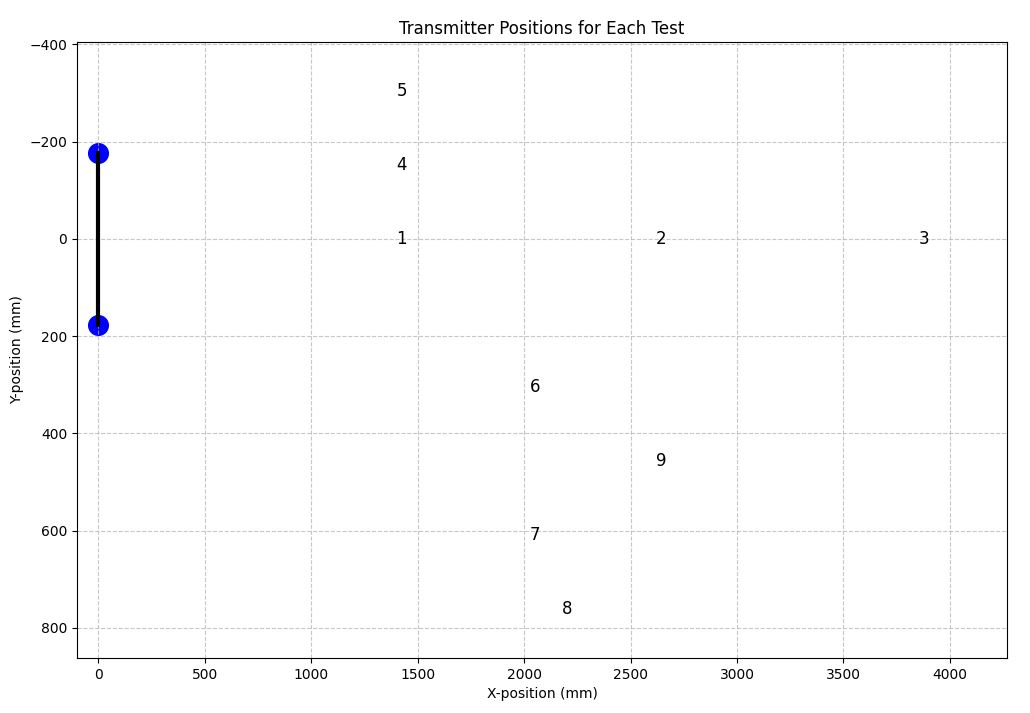
\includegraphics[width=\textwidth]{txpos}
	\caption{Transmitter position for each test}
	\label{fig:txpos}
\end{figure}

Note that the z-coordinate is relatively constant across the nine tests, but differs slightly (as will be seen in future plots). Different boxes were used to support the transmitter between some of the tests; the goal was to achieve the same z-position as the center of the receiver array. Additionally, the floor of the testing environment was slightly sloped at -1° along the x-axis and 0.5° along the y-axis relative to the test frame; this slope affects the true coordinates of the transmitter in the test frame. Figure \ref{fig:testpic} shows a picture of the testing environment.

\begin{figure}[htbp]
	\centering
	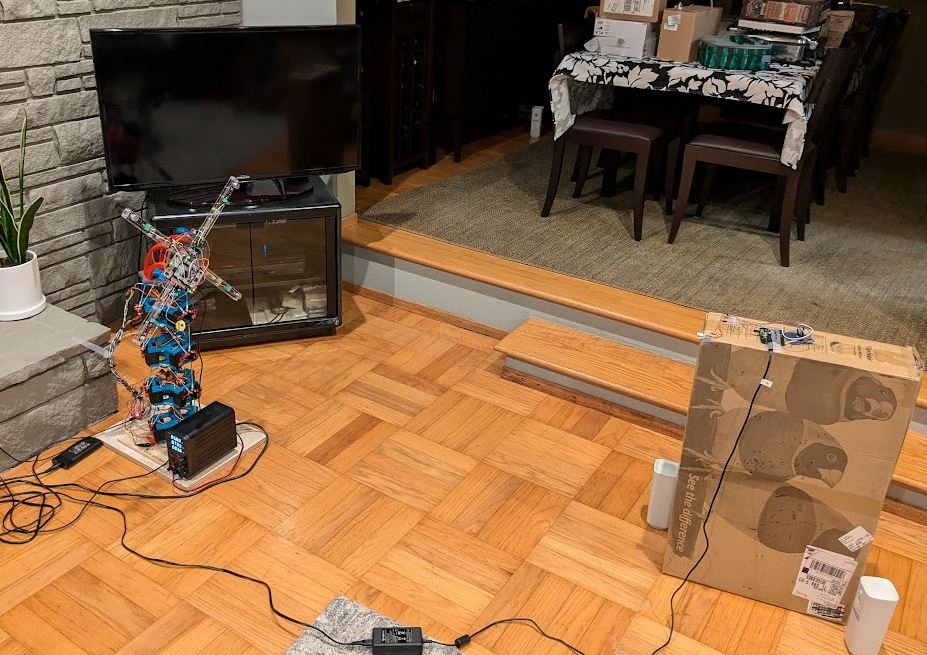
\includegraphics[width=0.9\textwidth]{testpic}
	\caption{Test environment for Test 5}
	\label{fig:testpic}
\end{figure}

The true position of the transmitter in each test was measured multiple times using a combination of rulers, yardsticks, measuring tape, and levels. The measurements account for the misalignment between the testing environment floor and the test frame of the Fo-SHIP. The transmitter position was measured three times for each test, and the listed transmitter position is the average of the three position estimates. The estimated uncertainty in the true position of the transmitter is ±0.5cm; this uncertainty is primarily driven by the resolution of the measuring devices and potential angular misalignments between measurement devices. Additionally, it incorporates the range of individual measurements; none of the three measurements for each test exceeded this range.

Finally, for each transmitter position, three tests were performed: one stationary, one rapid movement, and one gradual movement. For the stationary tests, the Fo-SHIP remained at its home position and did not move between acoustic position estimates. These tests were the best for decoupling the Fo-SHIP position estimate inaccuracy (which remains constant in the test and does not contribute to the noise in position estimates) from the acoustic positioning system inaccuracy. For the rapid movement tests, the Fo-SHIP waits until an acoustic position estimate is formed (and transmitted from the STM32 to the ESP32), then moves to a new position in a short amount of time (\textless0.5s). For the gradual movement tests, the Fo-SHIP similarly waits until a new acoustic position estimate is formed and transmitted, and then moves to a new position slowly (\textgreater1.5s). The distinction between rapid and gradual movements was made to check for differences between the two Kalman filter models; would rapid movement (with high accelerations) provide a better dead reckoning estimate, and thus have the iSBL-SF KF perform better?

\section{Results and System Accuracy} \label{sec:6s2}
The testing was performed over the course of a week, with a total of 30 hours of active testing taking place. A total of 21572 position estimates were formed, with 10304 estimates from stationary tests and 11268 from moving tests (5371 rapid and 5897 gradual). In this section, one main type of plot will be shown: y- vs z-differences for a particular test location (or group of test locations). The differences are defined as the estimated position (as calculated by one of the three methods) minus the true position of the receiver array for that datapoint (calculated using the Fo-SHIP setpoint and forward kinematics model). The x-difference is purely dependent on the simulated depth measurements, so showing it would be unnecessary. All plots of this type share the same (equal) axes; the position estimation accuracy between two plots can be compared visually. Code for generating these plots using any number of test locations, type of tests, and axes of movement (if only z-axis movement is desired, for example) can be found in the GitHub repository for this thesis \cite{thesisgit}.

The “accuracy” of the position estimate has two components: the mean difference (the average difference between the real and estimated position along an axis) and the standard deviation of differences. The mean difference can be thought of as the difference between the true position and the model’s position estimate, neglecting the effects of random noise. The standard deviation can be thought of as the noise surrounding that average. The mean difference is a good benchmark for the absolute accuracy of the system over time, and depends on absolute factors in the system design (misalignments / incorrect measurements between acoustic receivers, errors in the algorithm, and uncertainty in the true position of the transmitter). The standard deviation is a good benchmark for the inaccuracy in a single position estimate, and depends on transient variables (inconsistent speed of sound in air, noisy sounds in the testing environment, and error in the Fo-SHIP’s position estimate as it moves around).

\subsection{Distance versus Accuracy} \label{ssec:6s2s1}
In general, tests that were further away had much more spread in the position estimates; this trend holds across all three types of tests (stationary, rapid movement, gradual movement). This matches expectations: as the distance between the transmitter and receiver array increases, the signal-to-noise ratio of the received signals drops significantly. This lowers the accuracy of the time-differencing between signals, which produces a less accurate acoustic position estimate. Additionally, the acoustic position system is primarily computing the vector between the receiver array and the transmitter; as the distance to the transmitter increases, the error in the direction of this vector has a greater effect on the position estimate. Figure \ref{fig:d_3_s_nomu} shows the stationary results for Test 3, which had the largest distance between the transmitter and receiver array; Figure \ref{fig:d_4_s_nomu} shows the stationary results for Test 4, which had one of the smaller distances between the transmitter and receiver array. Note the massive decrease in the spread of the position estimates, as well as the smaller standard deviations in each model; as distance increases, the standard deviation of the differences increases.

\begin{figure}[htbp]
	\centering
	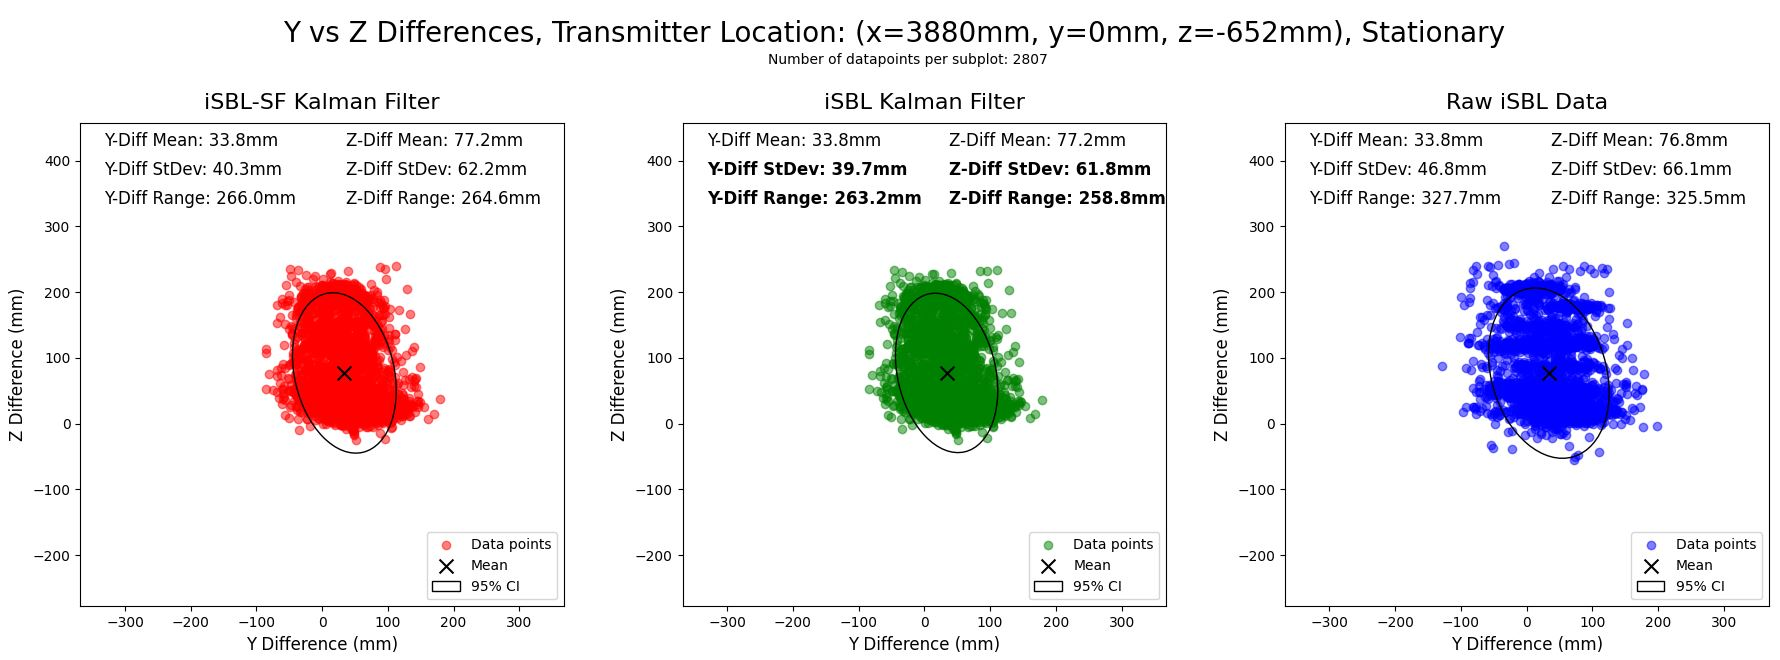
\includegraphics[width=\textwidth]{d_3_s_nomu}
	\caption{Stationary results for Test 3 (transmitter far away)}
	\label{fig:d_3_s_nomu}
\end{figure}

\begin{figure}[htbp]
	\centering
	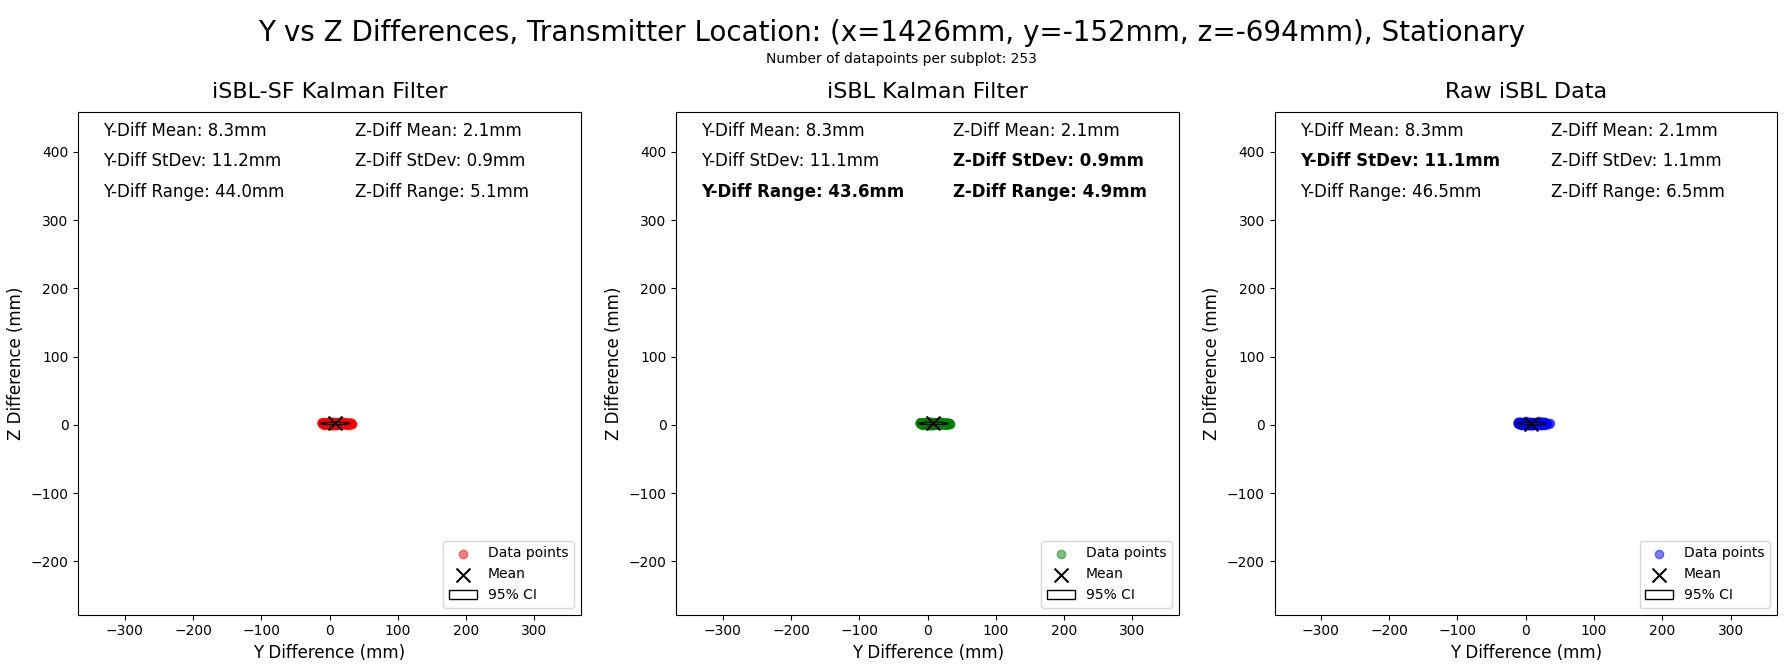
\includegraphics[width=\textwidth]{d_4_s_nomu}
	\caption{Stationary results for Test 4 (transmitter close up)}
	\label{fig:d_4_s_nomu}
\end{figure}

The average standard deviation across the three models was calculated for each testing location and the results were plotted in Figure \ref{fig:distvsstd}, comparing the standard deviation to the distance between the transmitter and receiver array. A power trendline was chosen for both axes; it was assumed that the inverse square law of sound propagation (sound volume / power decreases relative to the square of the distance from the transmitter) would be the primary force in the increased inaccuracy of the estimates; however, the error also increases linearly with distance due to the acoustic positioning system's angle-based position estimate method, as described in the previous paragraph. Note that the standard deviation of differences is scaled to account for the angle between the transmitter and receiver array for that test; tests with zero angle are unaffected, while tests with a large angle have their standard deviations scaled linearly to account for the effect of the angle on the accuracy of the tests. For future implementations, it is recommended to compensate for the perceived volume at the receiver (according to the inverse-square law and sound attenuation factor).

\begin{figure}[htbp]
	\centering
	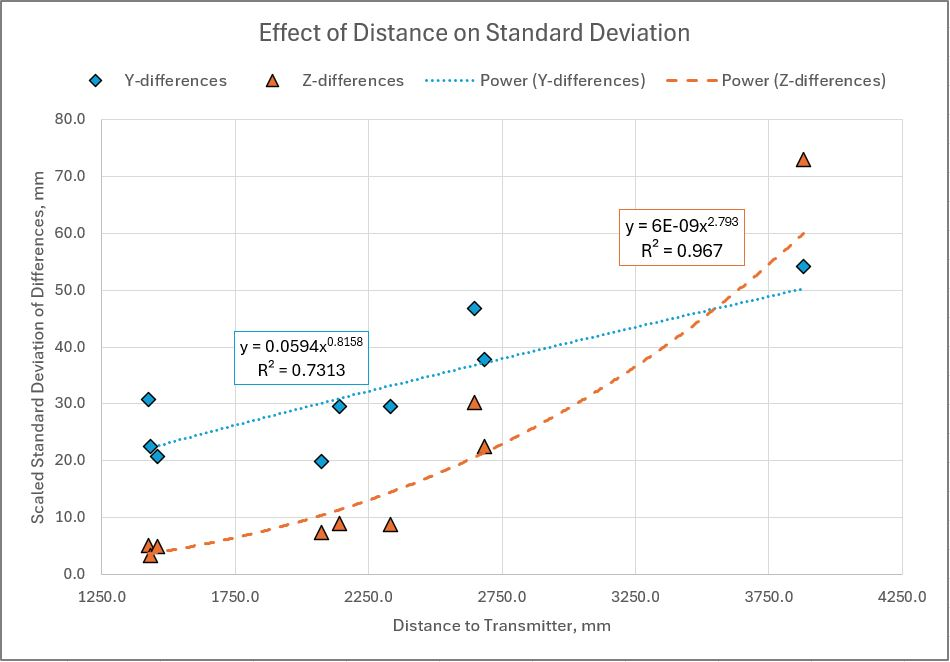
\includegraphics[width=.95\textwidth]{distvsstd}
	\caption{Standard deviation of all tests as a function of distance to transmitter, fit to power trendline}
	\label{fig:distvsstd}
\end{figure}

For this limited testing, the z-differences tended to fit this model well, while the y-differences did not. The main reason for this is assumed to be the large yaw angle inaccuracy in the orientation estimate of the system. The magnetometer was by far the most inaccurate sensor in the IMU; the earth’s magnetic field is quite weak compared to the strong magnetic fields produced by the 24 servo motors and other electrical circuitry near the IMU. As described in Section \ref{sec:6s4}, the yaw angle was only accurate to within about ±2°. This inaccuracy in the y-axis is very prevalent in other tests, particularly those performed near the middle of the operating range of the system (1, 2, 4, 5, 6, and 9).

\subsection{Angle versus Accuracy} \label{ssec:6s2s2}
The angle between the x-axis of the test frame and the vector pointing from the origin to the transmitter location had a minimal effect on the accuracy of the three methods. It was presumed that the high directionality of the receivers (as described in Section \ref{3s4}) would have a large impact on the accuracy of the position estimates; as the angle between the transmitter and receiver array increases, the signal-to-noise ratio at the receiver decreases. However, this did not seem to be the case. As long as the receivers could hear the transmitter (which was the case below angles of 19.1°), the angle had little impact on the standard deviation. Figure \ref{fig:d_8_r_nomu} shows the results of the rapid movement test for Test 8 with the largest angle of 19.1°; Figure \ref{fig:d_2_r_nomu} shows the results of the rapid movement test for Test 2 with an angle of 0°. Both tests have a similar distance, with Test 2 being about 12\% further away than Test 8. Test 8 appears to have slightly more spread among the y-differences, but this can likely be attributed to the increase in distance compared to Test 2. 

\begin{figure}[htbp]
	\centering
	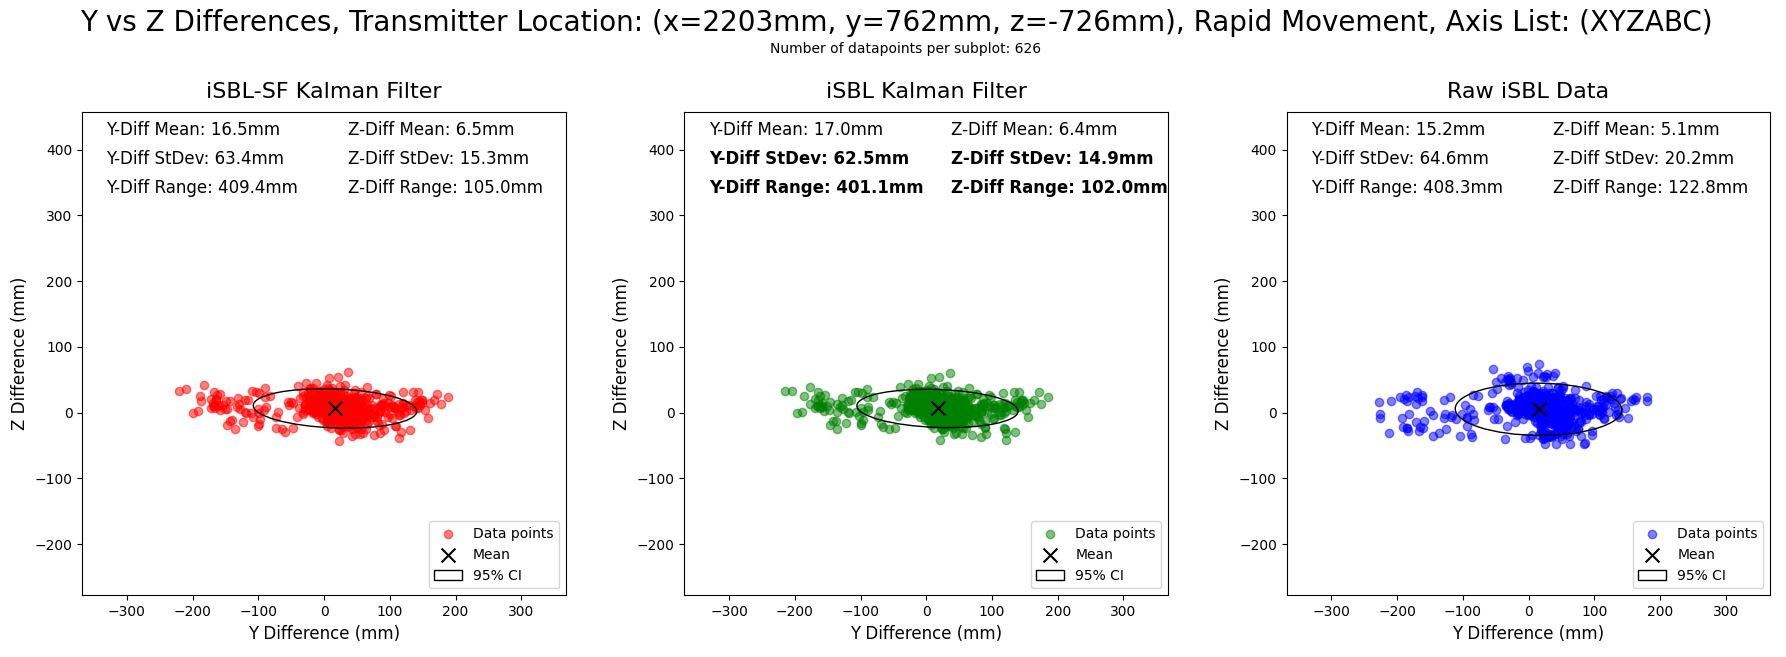
\includegraphics[width=\textwidth]{d_8_r_nomu}
	\caption{Rapid movement results for Test 8 (large angle between transmitter-origin vector and x-axis)}
	\label{fig:d_8_r_nomu}
\end{figure}

\begin{figure}[htbp]
	\centering
	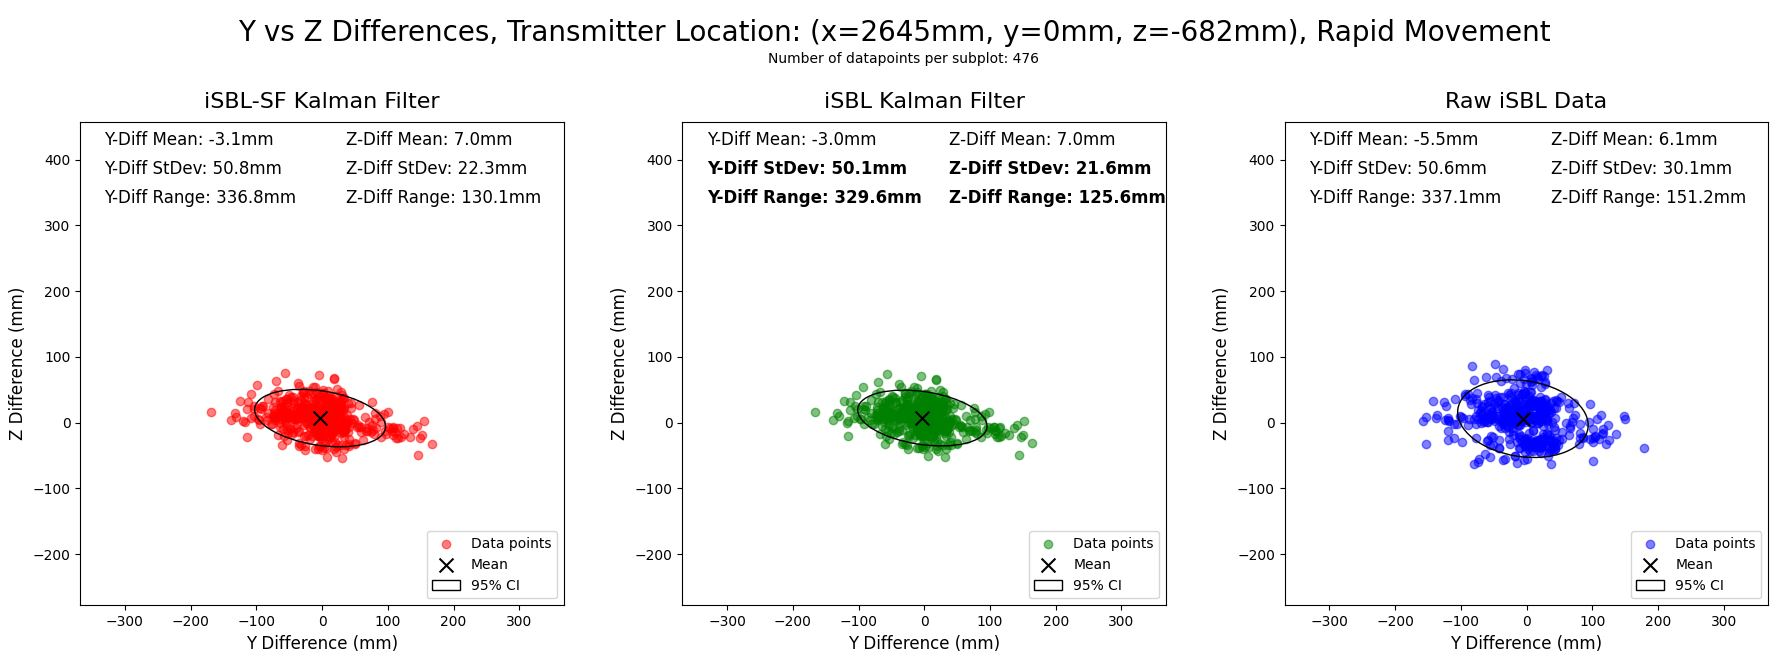
\includegraphics[width=\textwidth]{d_2_r_nomu}
	\caption{Rapid movement results for Test 2 (zero angle between transmitter-origin vector and x-axis)}
	\label{fig:d_2_r_nomu}
\end{figure}

The average standard deviation of differences for each test was plotted against the angle between the transmitter-origin vector and the x-axis of the test frame; the results can be seen in Figure \ref{fig:yawvsstd}. Note that similar to the last subsection, the standard deviations here are scaled to account for distance. The data for both axes was fitted to linear trendlines, with much lower correlation values than the distance versus standard deviation trendlines in the previous subsection.

\begin{figure}[htbp]
	\centering
	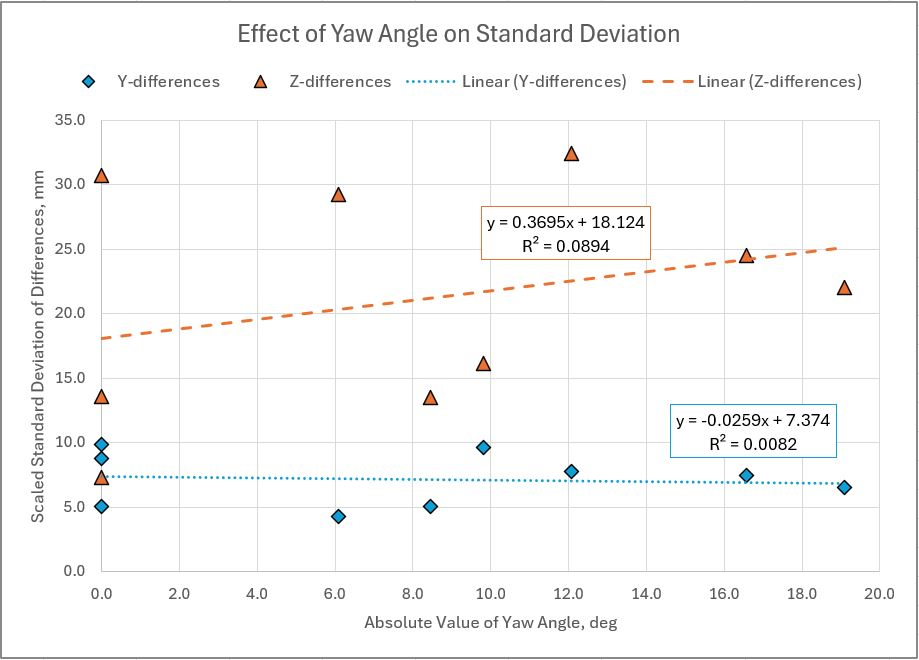
\includegraphics[width=\textwidth]{yawvsstd}
	\caption{Standard deviation of all tests as a function of angle between transmitter-origin vector and x-axis, fit to linear trendline}
	\label{fig:yawvsstd}
\end{figure}

\subsection{Stationary Tests versus Moving Tests} \label{ssec:6s2s3}
Stationary tests produced much less noise than moving results across all testing locations. This is expected: in moving tests, the uncertainty in the Fo-SHIP ground-truth position estimate (which grows as the angle of the Fo-SHIP increases) adds to the noise of the acoustic position estimate. Stationary tests are a good representation of the accuracy of the acoustic positioning system alone (with the y-axis being affected significantly by yaw inaccuracies of the magnetometer, while the z-axis is much less affected); moving tests are a decent representation of a real underwater implementation of the system (incorporating motion into the results), but are clouded by the inaccuracy of the Fo-SHIP position estimate. Figure \ref{fig:d_6_s_nomu} shows the stationary test results for Test 6, while Figure \ref{fig:d_6_rg_nomu} shows the moving test results for the same position (rapid and gradual).

\begin{figure}[htbp]
	\centering
	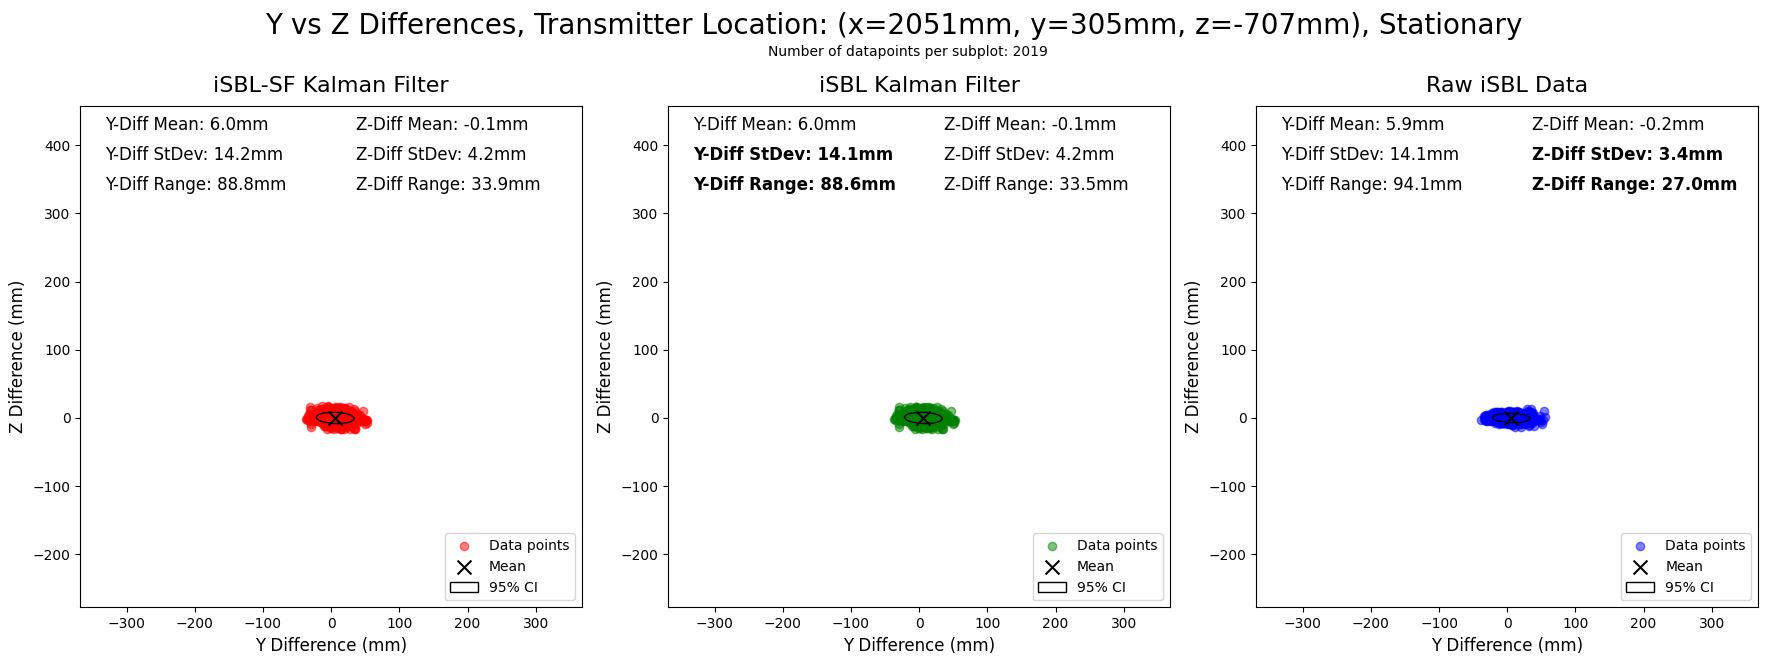
\includegraphics[width=\textwidth]{d_6_s_nomu}
	\caption{Stationary results for Test 6}
	\label{fig:d_6_s_nomu}
\end{figure}

\begin{figure}[htbp]
	\centering
	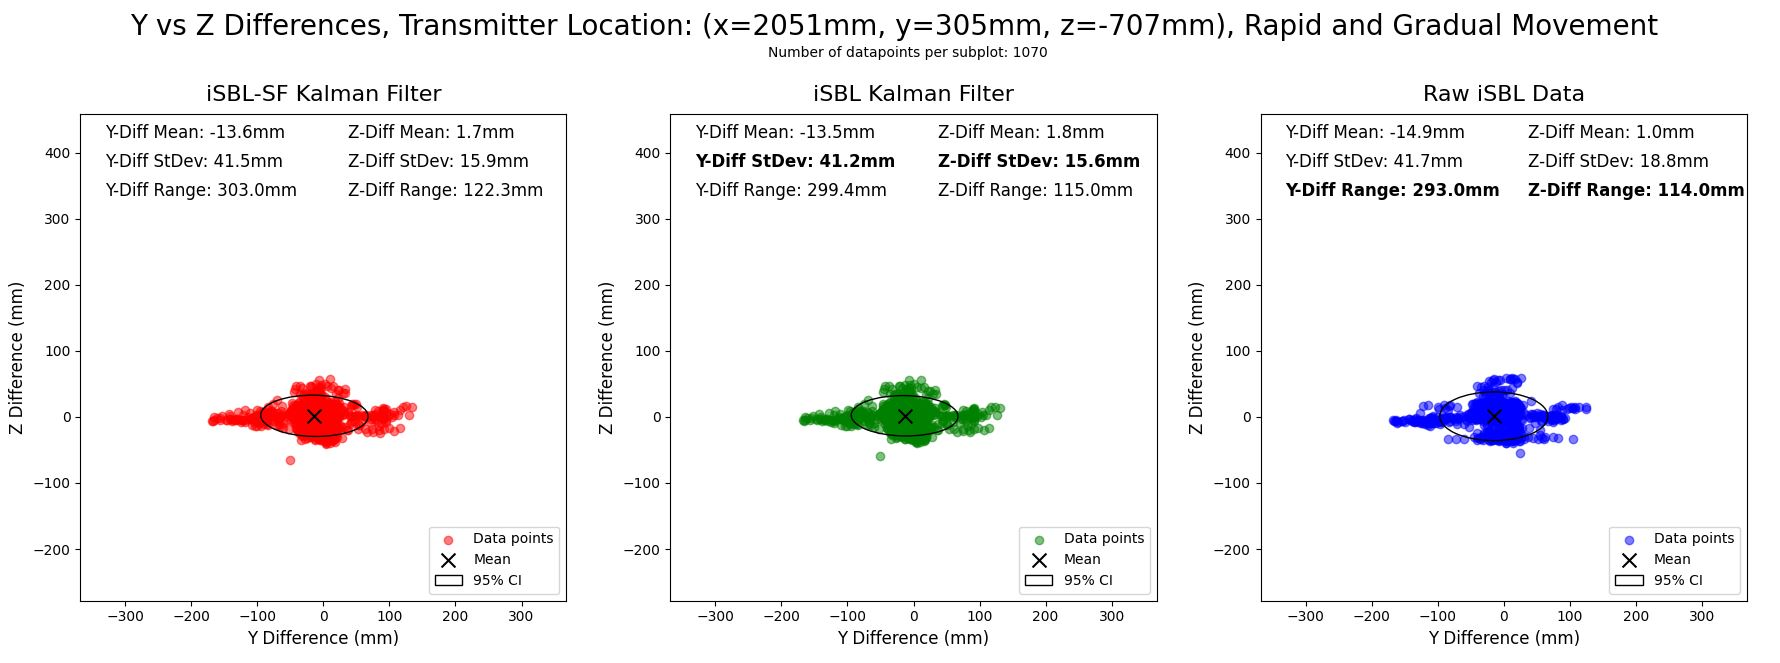
\includegraphics[width=\textwidth]{d_6_rg_nomu}
	\caption{Moving results for Test 6 (combined rapid and gradual movement)}
	\label{fig:d_6_rg_nomu}
\end{figure}

The difference in accuracy between stationary and moving tests is not limited to individual test locations. Figure \ref{fig:d_all_s} shows the stationary test results for all nine tests (with means subtracted to provide better comparison), and Figure \ref{fig:d_all_rg_xyzabc} shows the moving test results for all nine tests (combined gradual and rapid movement, means subtracted). The moving tests show a significant increase in spread of the y-differences. Note that the ellipse in each plot shows the 95\% confidence interval for the tests and is a better representation of the average measurement given the large sample size for these plots.


\begin{figure}[htbp]
	\centering
	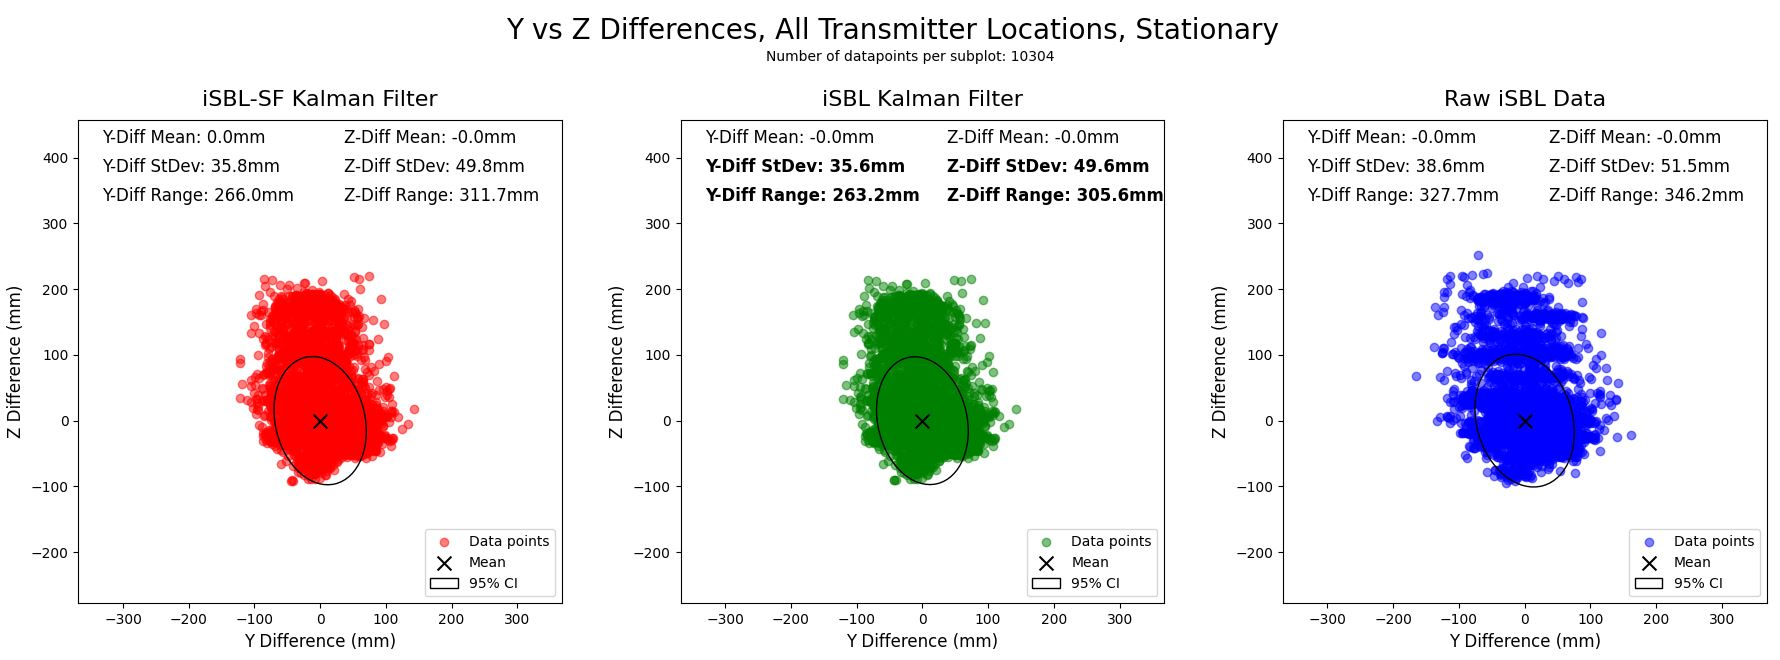
\includegraphics[width=\textwidth]{d_all_s}
	\caption{Stationary results for all test locations}
	\label{fig:d_all_s}
\end{figure}

\begin{figure}[htbp]
	\centering
	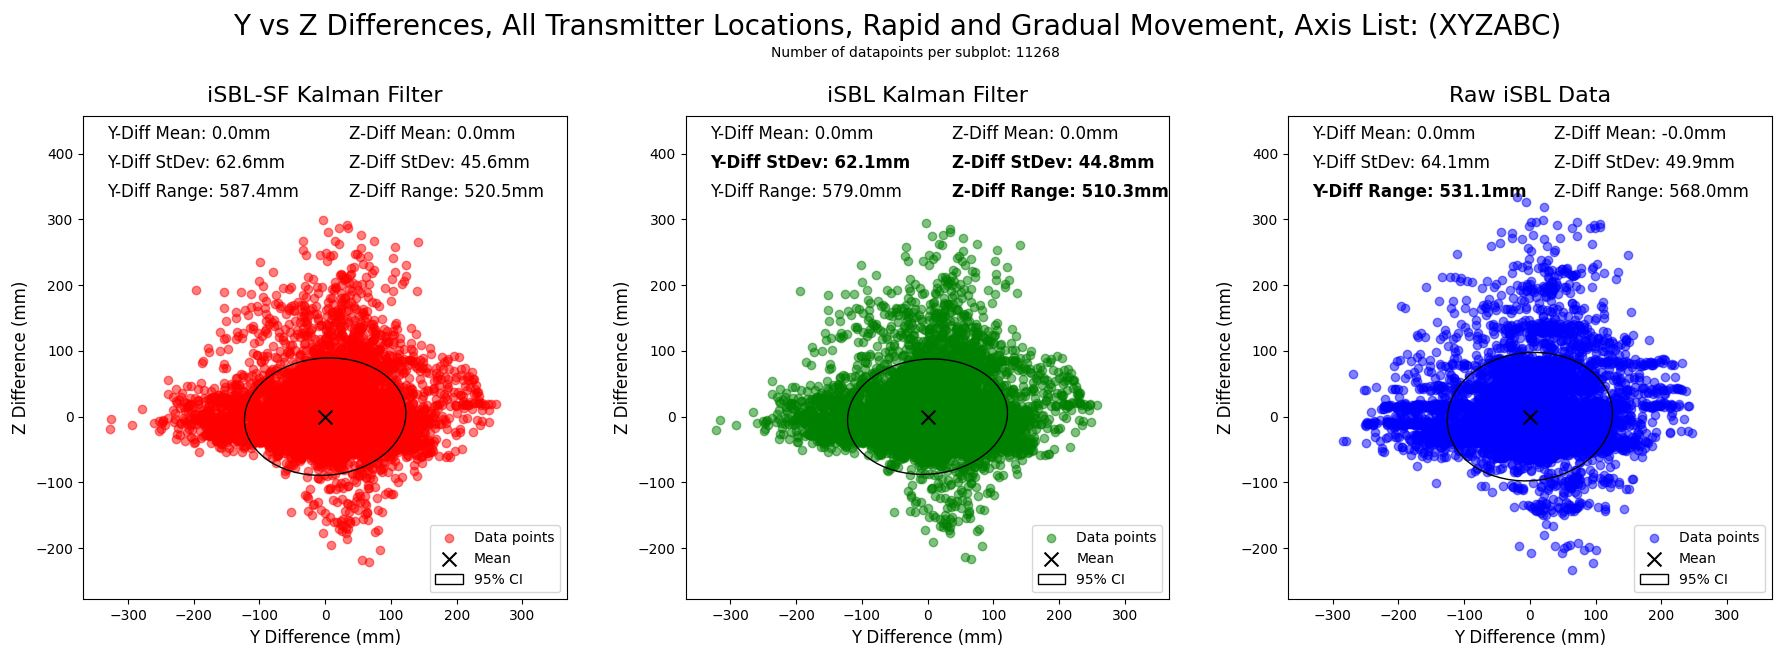
\includegraphics[width=\textwidth]{d_all_rg_xyzabc}
	\caption{Moving results for all test locations (combined rapid and gradual movement)}
	\label{fig:d_all_rg_xyzabc}
\end{figure}

\subsection{Rapid Movement versus Gradual Movement} \label{ssec:6s2s4}
Rapid and gradual movement tests had very similar results; the primary reason for the separation of these movement types (as opposed to one “moving” test category) was to elicit a difference between the iSBL-SF and iSBL Kalman filters. It was hypothesized that rapid movement, which includes much greater accelerations, would provide a better dead reckoning change-in-position estimate than gradual movement. This was proven incorrect; the iSBL-SF model was never more accurate than the iSBL model. Figure \ref{fig:d_all_r_xyzabc} shows the results for all rapid tests (means subtracted), and Figure \ref{fig:d_all_g_xyzabc} shows the results for all gradual tests (means subtracted). 

\begin{figure}[htbp]
	\centering
	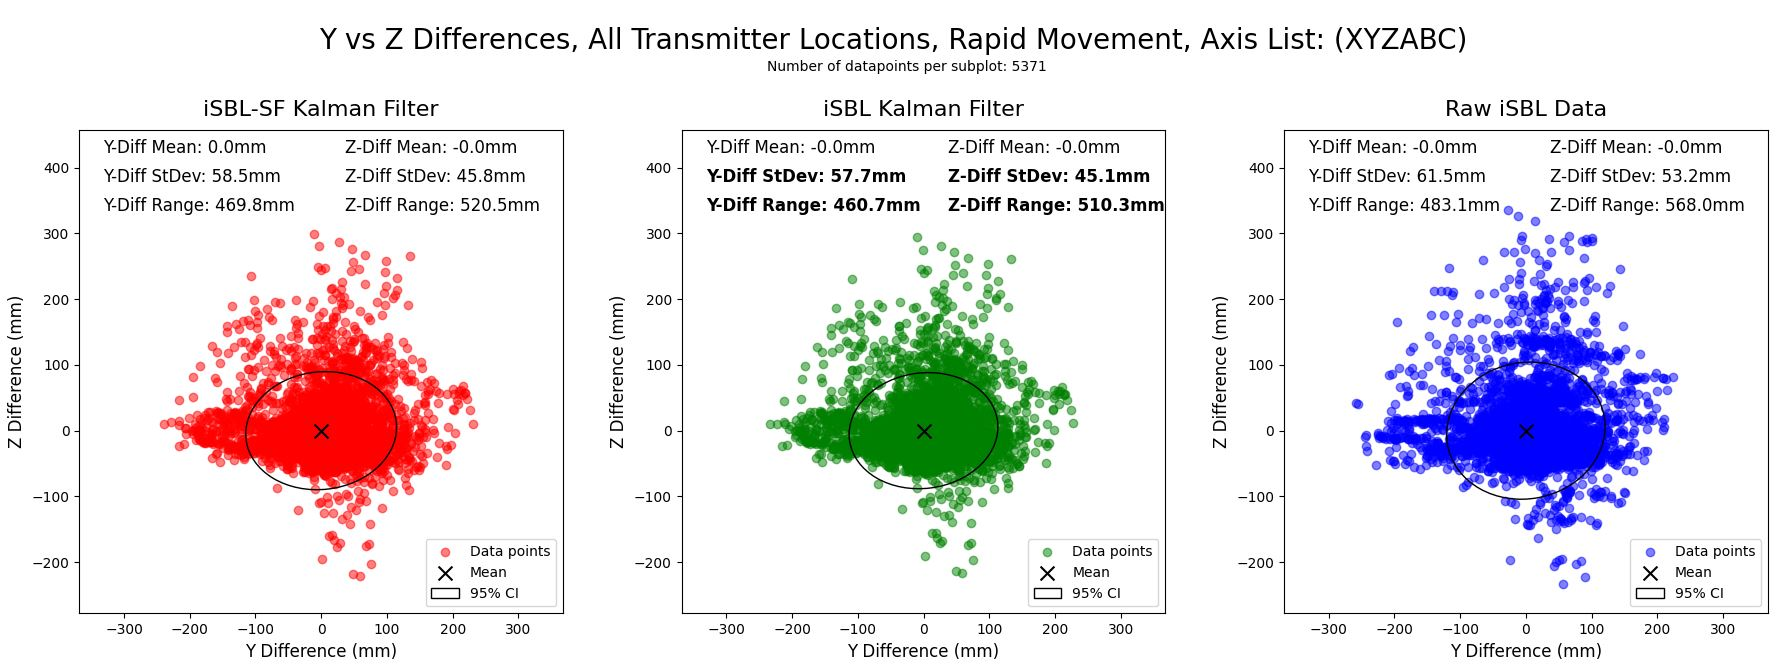
\includegraphics[width=\textwidth]{d_all_r_xyzabc}
	\caption{Rapid movement results for all test locations}
	\label{fig:d_all_r_xyzabc}
\end{figure}

\begin{figure}[htbp]
	\centering
	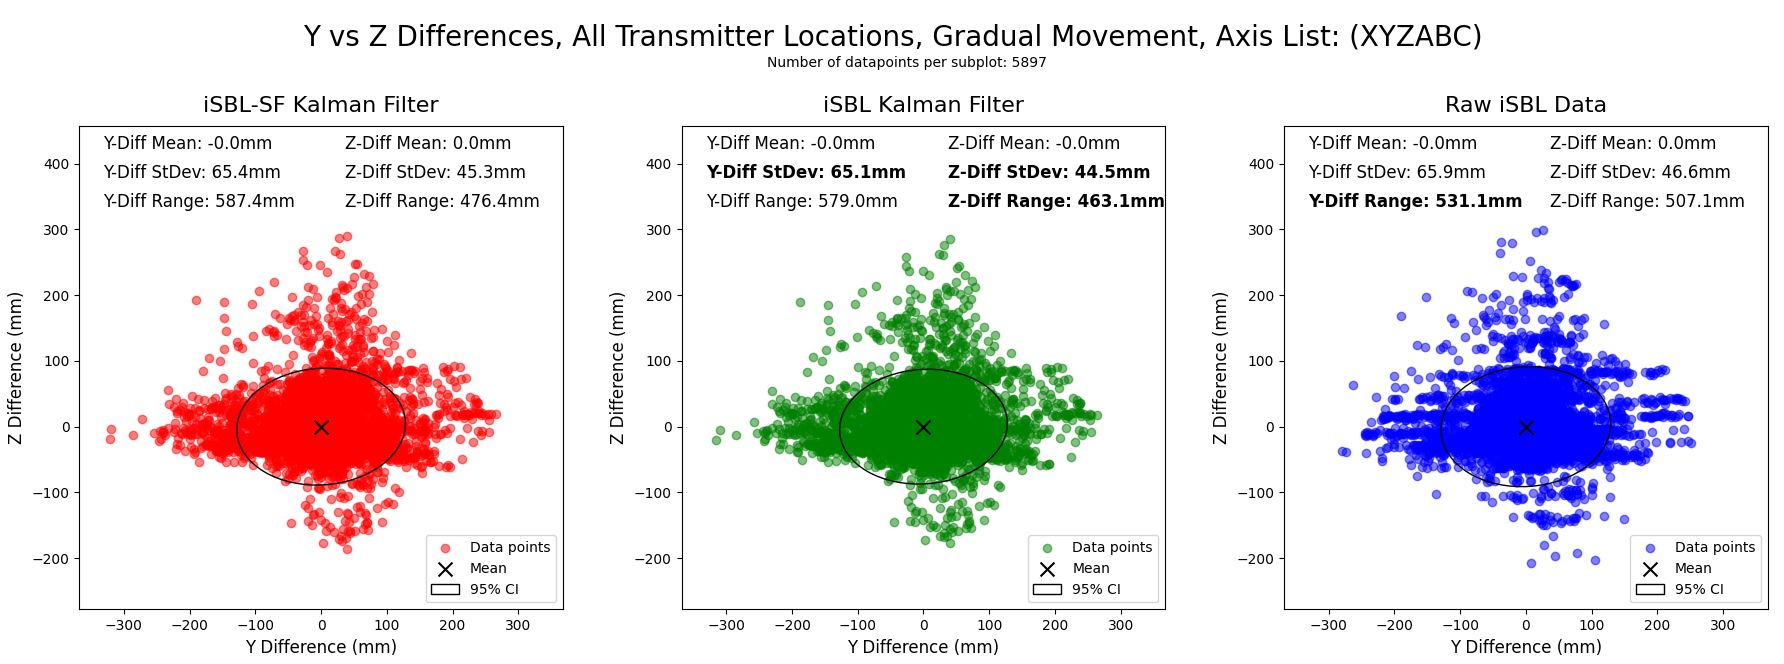
\includegraphics[width=\textwidth]{d_all_g_xyzabc}
	\caption{Gradual movement results for all test locations}
	\label{fig:d_all_g_xyzabc}
\end{figure}

Discrepancies between the gradual and rapid tests can mostly be attributed to three factors: 
\begin{itemize}[noitemsep,topsep=0pt,]
	\item Rapid and gradual movements cause different hysteresis errors in the servo motors, leading to different ground-truth position estimate errors
	\item Rapid movements might provide better orientation estimates given the higher angular velocity and acceleration of the movements
	\item Rapid tests used a larger step size between different positions; gradual movement tests often used increments of 1mm / 1° between set points, while rapid movement tests often used increments of 4mm / 4°
\end{itemize}

\subsection{Normality of Results} \label{ssec:6s2s5}
The Kalman filter algorithm assumes normally-distributed noise for both measurements and state estimates \cite{kalman}. The normality of the dead reckoning change-in-position measurements will not be evaluated here; not enough data was collected using raw dead reckoning data to evaluate the normality, and the system is not accurate enough to be worth analyzing at its current state. The normality of the acoustic positioning system estimates - the raw iSBL data used as measurements for both Kalman filters - can be considered. Additionally, the normality of the state estimate of each Kalman filter can definitely be considered.

Figure \ref{fig:h_all_rgs} shows histograms of the differences for the y- and z-axes for all data points (all testing positions, stationary, rapid movement, and gradual movement results combined). The y-differences appear to loosely fit the normal distribution, while the z-differences are much more skewed. This phenomenon is present across all test positions and types; Figure \ref{fig:h_3_s} shows the histograms for stationary estimates of Test 3 (the furthest position), and Figure \ref{fig:h_4_s} shows the histograms for stationary estimates of Test 4 (one of the closest positions). 

For positions not at the edge of the acoustic positioning system’s range, the z-differences for the Kalman filters (the state estimates) become fairly normally-distributed; for far-away positions, the z-differences skew heavily. The raw acoustic position estimates (the measurements for the Kalman filters) tend to be relatively normal in the y-differences, but the z-differences show significant banding. This banding is a result of the time-differencing in the acoustic positioning system. The FFT cross-correlation tends to choose time differences that align the peaks of the two signals. This results in a “banding” effect, where the shift between the peaks is highly related to the wavelength of the transmitted sound. Using a higher frequency (like 200kHz) would very likely bring these peaks closer together.

This banding is mostly present in the middle-range of the iSBL system; as the distance increases, the noise in the orientation estimate has a greater effect on the position estimate error. Also, note that there is almost zero banding in the y-differences! The y-difference error is primarily driven by the orientation estimate error from the magnetometer, so the banding is much less pronounced. 

\begin{figure}[htbp]
	\centering
	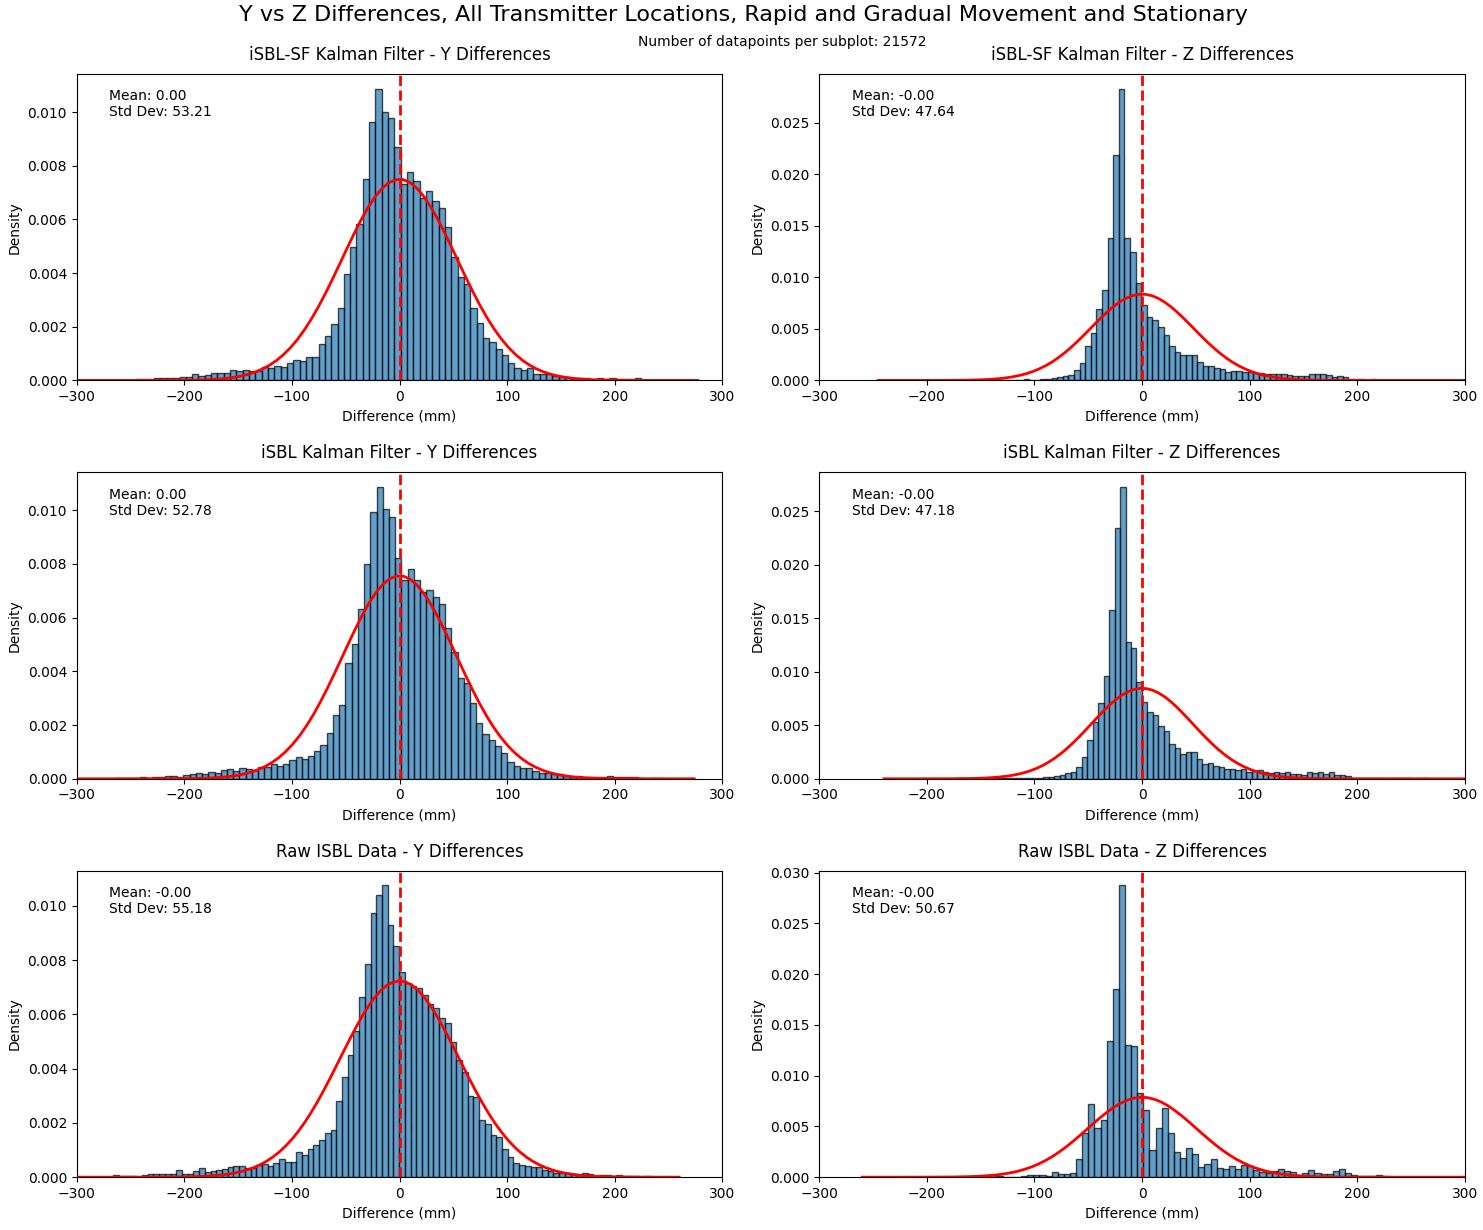
\includegraphics[width=\textwidth]{h_all_rgs}
	\caption{Histograms of differences for all test locations}
	\label{fig:h_all_rgs}
\end{figure}

\begin{figure}[htbp]
	\centering
	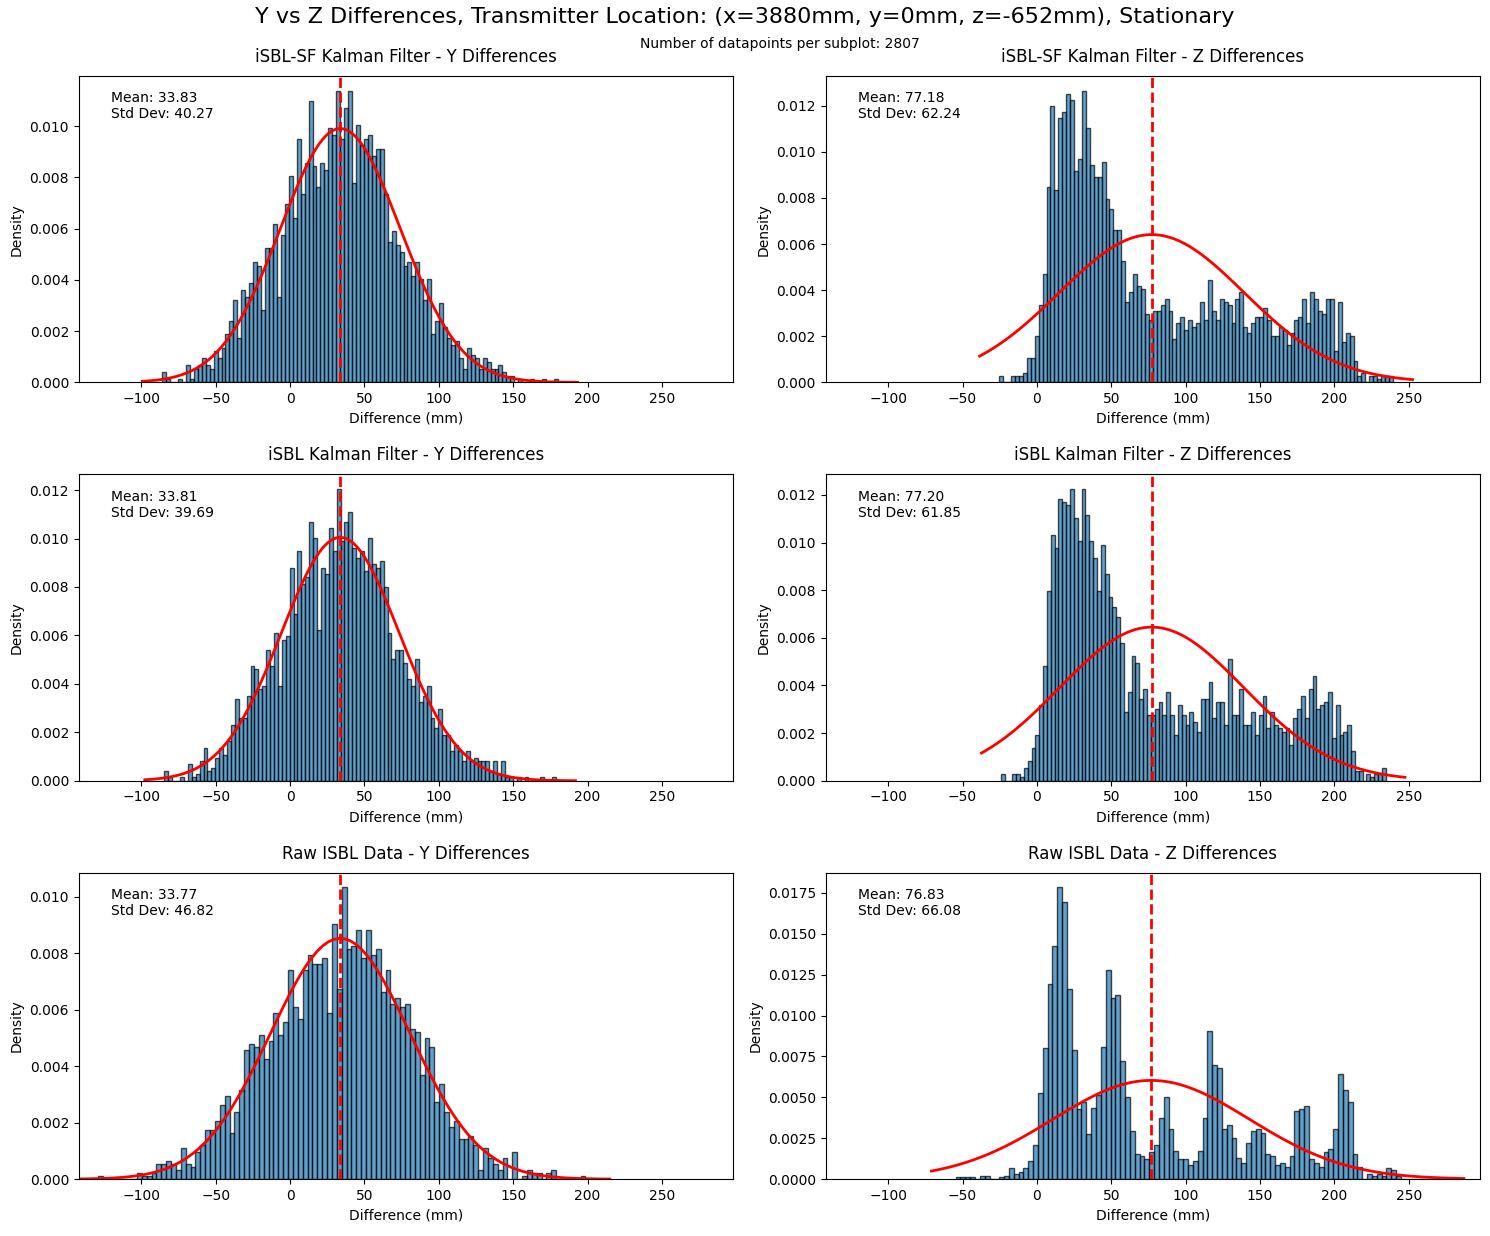
\includegraphics[width=\textwidth]{h_3_s}
	\caption{Histograms of differences for Test 3 (transmitter far away), stationary results only}
	\label{fig:h_3_s}
\end{figure}

\begin{figure}[htbp]
	\centering
	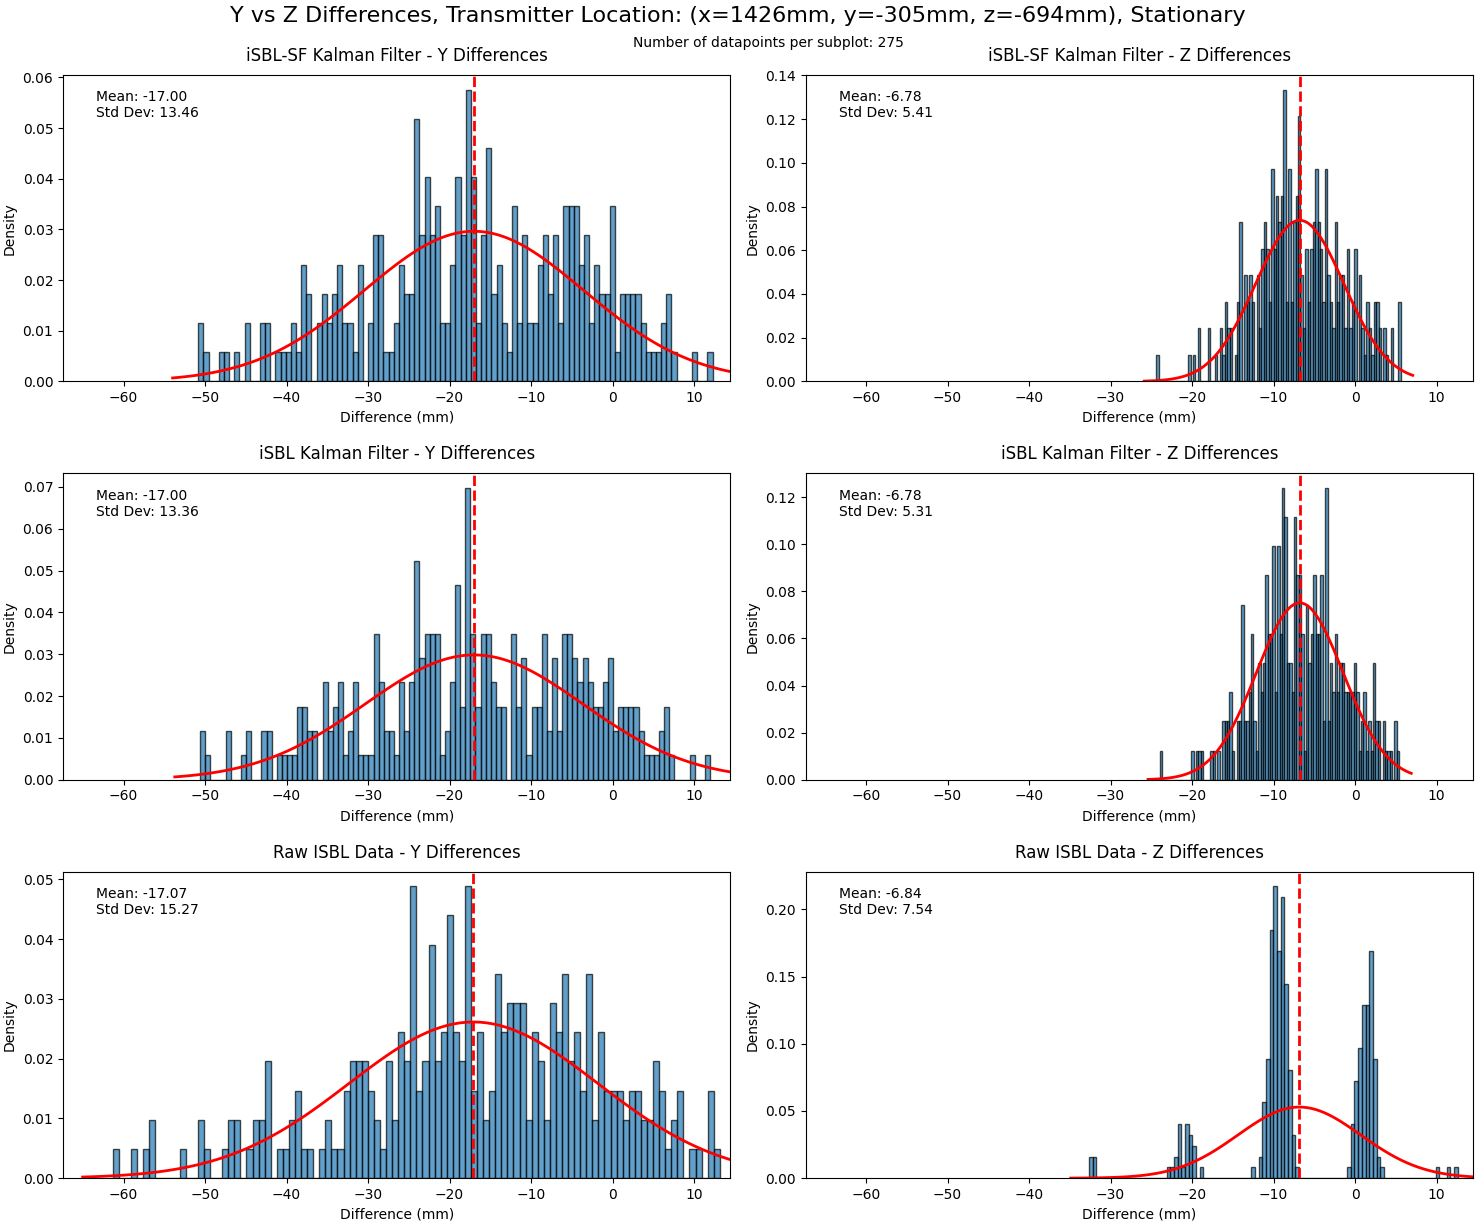
\includegraphics[width=\textwidth]{h_4_s}
	\caption{Histograms of differences for Test 4 (transmitter close up), stationary results only}
	\label{fig:h_4_s}
\end{figure}

\pagebreak

\subsection{Overall Accuracy and Best Model} \label{ssec:6s2s6}
A summary of all the testing results can be seen in Figures \ref{fig:datasum1} and \ref{fig:datasum2}. The row “All Combined, All Positions” provides the best overview of the overall accuracy of each model; other rows contain the results from individual testing locations (as well as the combined stationary, rapid movement, and gradual movement tests). The best model, the iSBL KF, had an average mean difference of 22.1mm (the average positional error between the true and estimated position) and an average standard deviation of differences of 49.9mm. The accuracy in the y-axis is slightly worse than that of the z-axis, primarily due to the magnetometer in the IMU. However, these estimates cannot be de-coupled from the uncertainty in the true position of the transmitter and receiver array; the uncertainty in the transmitter position is ±5mm as described in Section \ref{sec:6s1}, and the average uncertainty in the Fo-SHIP ground-truth position estimate is ±7mm as described in Section \ref{sec:2s6}. This means that the best model accuracy may be better than the average error of 22.1mm, but can only be estimated to that degree due to the ±12mm position uncertainty. A more-accurate ground-truth positioning system would allow for a better accuracy estimate of the iSBL system.

\begin{figure}[htbp]
	\centering
	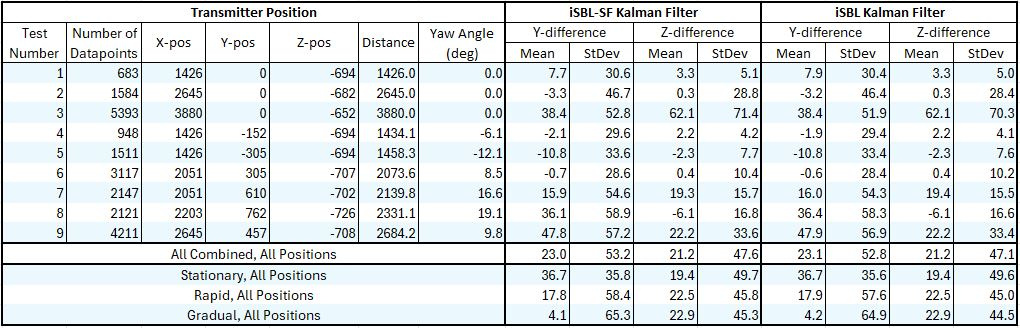
\includegraphics[width=\textwidth]{datasum1}
	\caption{Summary of data collection, iSBL-SF and iSBL Kalman filter models}
	\label{fig:datasum1}
\end{figure}

\begin{figure}[htbp]
	\centering
	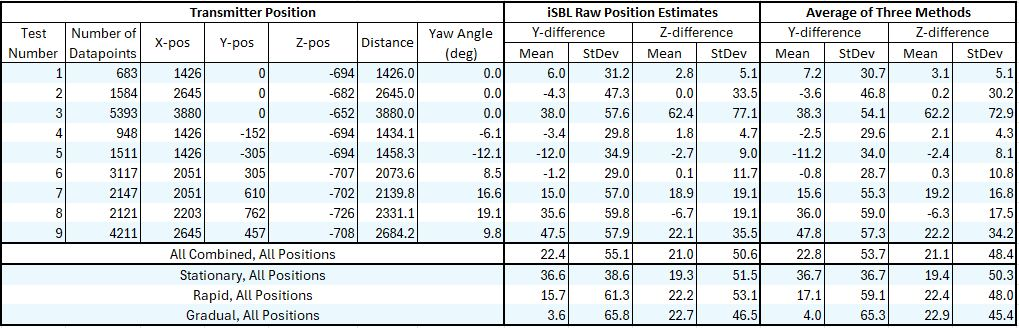
\includegraphics[width=\textwidth]{datasum2}
	\caption{Summary of data collection, raw iSBL data and average of three models}
	\label{fig:datasum2}
\end{figure}

The plots from the previous subsections also show that the iSBL Kalman filter tends to have the best accuracy. Here, the “best accuracy” is defined as the lowest standard deviation and range of the differences across the nine tests. The average difference of each model tends to be very similar; including a Kalman filter doesn’t change the average error from the true position for stationary tests, and it can actually cause a bit of error for moving tests (since the state estimate lags the measurements slightly). The noise component of the accuracy shows the largest variation between models. Generally, the Kalman filter models are better than the raw iSBL estimates at constraining the noise. The inclusion of dead reckoning data almost always hurt the position estimates, meaning that the iSBL-SF model was the worst of the three. With better dead reckoning data, it is very likely that the iSBL-SF model would outperform the other two.

\section{Extrapolation to Underwater Regime} \label{sec:6s3}
All of the work done in this thesis is above-water, but the ultimate goal is to implement the acoustic positioning system in an underwater environment on an AUV. Some assumptions were made for the above-water implementation that would not hold for an underwater implementation:
\begin{itemize}[noitemsep,topsep=0pt,]
	\item The speed of sound is 343 m/s in air
	\item The speed of sound is constant in air, so sound travels in a straight line
	\item The receiver array is located at some depth along the x-axis, and the depth can be simulated using the true x-coordinate of the transmitter and random noise
	\item Sound attenuates very quickly in air, severely limiting the range of the positioning system
	\item No living creatures are strongly affected by the sound of the acoustic positioning system in the current testing environment
\end{itemize}

The speed of sound is between 1490 m/s and 1530 m/s in water \cite{computational}; this means that the speed of sound can be up to 4.47x faster in water than in air. Keeping the sampling rate the same at 851.4kHz, the maximum distance error for the time-differencing of two signals is 0.201mm in air or 0.899mm in water. This maximum error is directly related to the acoustic positioning system accuracy and (very roughly) translates to 4.47x worse positional accuracy compared to the above-water implementation. To keep the same level of accuracy underwater (particularly, keeping the standard deviation of the acoustic position estimates the same as this above-water prototype), the sampling rate for each microphone would need to be increased to 3.806MHz. It should be noted that this is an approximation - the relationship between the time-differencing of signals and the acoustic position estimate is highly complex. However, this approximation aims to show that the accuracy of an underwater implementation will be worse than the accuracy of this above-water prototype unless the sampling rate of the ADCs is increased by a significant factor.

The speed of sound is not constant in water and depends on depth, salinity, and temperature \cite{computational}. The speed of sound is not constant in air either; 343 m/s is just a convenient average, and the speed of sound in air varies orders of magnitude less compared to the speed of sound in water. The non-constant speed of sound in water would bend the path that sound takes underwater, just like light is bent when it transitions from air to water (like in a swimming pool or a glass of water). The current model assumes that sound travels in a straight line and that the distance between the transmitter and a receiver equals the time of arrival of the pulse times the speed of sound; this model is represented in the function \verb|calculate_toa()| as described in Section \ref{ssec:3s9s2}. This model would need to be modified to account for the way that sound bends in water, and the book \textit{Computational Ocean Acoustics} provides fantastic resources for implementing this change into the model \cite{computational}.

The above-water implementation simulates the “depth” of the receiver array along the x-axis; this made it possible to perform testing horizontally, as opposed to hanging the transmitter vertically above the Fo-SHIP and receiver array. However, this is not how the underwater system would work. Assuming the same North-East-Down frame, the depth of the array would be represented in the z-axis. This does not seem like a big change, but one major source of error becomes effectively doubled: the yaw component of the orientation estimate. Note that from Section \ref{sec:6s2}, yaw (driven primarily by the magnetometer) is the most inaccurate component of the IMU’s orientation estimate. Yaw does not affect the accuracy of the z-axis position estimate, which is one of two axes being estimated in the above-water prototype (depth provides the x-axis measurement). However, in the underwater system, the two axes being estimated are the x- and y-axis. This means that the yaw error will propagate to both axes being measured! It would be highly recommended to purchase a more accurate and precise magnetometer for an underwater implementation. Additionally, a depth sensor would need to be purchased to truly measure the depth of the array (and not just simulate it, as done in this implementation).

So far, the assumptions made for the above-water system have made the future underwater implementation less accurate. However, there is one benefit to using sound for underwater positioning: sound travels much further in water than in air for the same transmission power. Sound transmission (assuming planar waves, the standard model) decays according to the function in Equation \ref{eq:6eq1} \cite{computational}:

\begin{equation} \label{eq:6eq1}
	A(x) = A_0 e^{-\alpha x}
\end{equation}

Where \(A_0\) is the root-mean-square amplitude of the transmission volume at x=0, \(\alpha\) is the attenuation factor, and \(x\) is the distance from the transmitter. This attenuation factor depends on the frequency of the sound wave and the properties of the transmission medium. In the above equation, \(\alpha\) is in units of nepers/m; it is commonly represented in units of dB/m using the equations below \cite{computational}.

\begin{equation} \label{eq:6eq2}
	Loss = -20log\frac{A}{A_0} \approx 8.686 \alpha x
\end{equation}

\begin{equation} \label{eq:6eq3}
	\alpha^{'} [dB/m] \approx 8.686 \alpha
\end{equation}

The attenuation factor of 40kHz sound in water is approximately 0.001 dB/m \cite{computational}, according to Figure \ref{fig:attenuation} in Section \ref{sec:3s4}; in air, the attenuation factor is approximately 128 dB/m, according to Figure \ref{fig:airatten} \cite{airatten}. Sound can travel roughly 6km in water before its transmission volume is cut in half; in air, this distance is 4.69cm. This means that the range of the acoustic positioning system is exponentially greater than this air-based prototype. 

\begin{figure}[htbp]
	\centering
	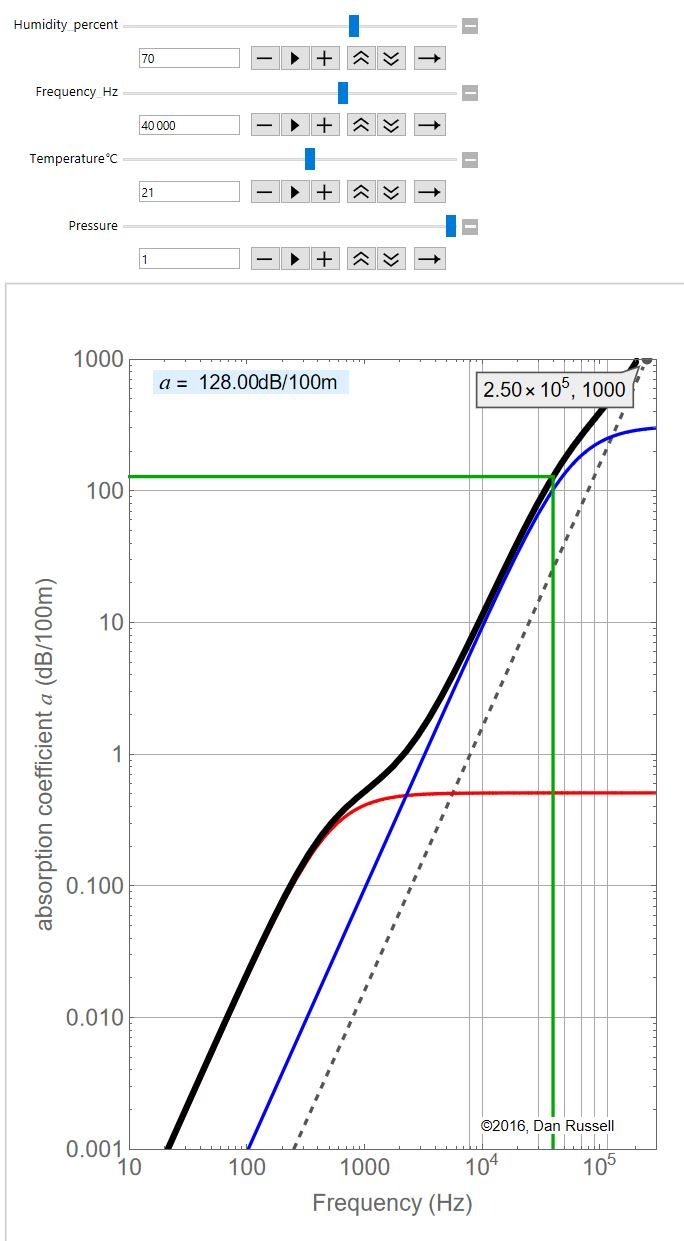
\includegraphics[width=0.7\textwidth]{airatten}
	\caption{Attenuation factor of 40kHz sound in air, room temperature and humidity \cite{airatten}}
	\label{fig:airatten}
\end{figure}

The effect of distance on the accuracy of the position estimate is not entirely negated; as described in Section \ref{ssec:6s2s1}, the acoustic positioning system primarily computes the vector between the transmitter and the receiver array; as distance increase, the error in this vector scales linearly. However, this much smaller attenuation factor will significantly improve the range of the underwater acoustic positioning system, and its importance cannot be understated.

Finally, only humans (and the occasional housecat) were near the acoustic positioning system during testing. The 40kHz pulses are outside of the audible range of humans, but a slight noise could be heard during each pulse: the “bits” encoded in the pulse (an 8-bit character, along with six header bits) are sent at 2kHz, which registers as a slight "clicking" noise. This noise was only noticeable to humans if the testing environment background noise was low. Note that the housecats seemed unaffected by the noise and did not respond to interview requests regarding the noise level. However, it would be inappropriate to suggest implementing this system underwater without discussing the potential impacts on underwater wildlife.

Some research has been done on the effects of ultrasonic sound on marine life, but surely not enough. Russian researchers studied the effects of ultrasound equipment (500W, 27kHz) on fish species found in the Black Sea. They subjected the fish to the ultrasound for one hour per day over three days, and had the ultrasonic equipment at a distance of 10cm-30cm from the fish. They found slight behavioral changes in some of the fish, but observed no permanent physiological or biochemical changes when compared to the control group \cite{blacksea}.

Two marine acoustics researchers wrote a report discussing the impact of underwater sounds on various forms of marine life. They note that regulations and research in this field are sparse, and they present some guidelines for keeping marine life safe when working with sound underwater. Maximum and average sound pressure levels are specified in the paper, and the hearing ranges of many marine animals are given - notably, many fish hearing ranges appear to be below 5kHz, far below ultrasonic frequencies. Still, staying below the sound pressure levels in this paper would be recommended for an underwater implementation \cite{assessing}.

A NOAA technical memorandum, published in 1998, presents work on marine mammal auditory systems. The author notes that some species of marine mammals, particularly of the parvorder Odontocetes (dolphins, toothed whales, etc.) have hearing ranges up to 200kHz. Many mammals in this parvorder can produce sound with intensities up to 200 dB re 1 \(\mu\)Pa in the ultrasonic range. The paper goes into much more detail on the mechanism of mammal auditory systems and the ranges of each individual species \cite{implications}. Ultrasonic frequencies produced by an acoustic positioning system (or SONAR), if kept below the intensities that mammals can produce, would likely not cause harm to the mammals; however, it may certainly disrupt their behavior.

Oceanographers found that ultrasonic antifouling devices (used to limit marine growth on the hulls of ships) have been negatively impacting beaked whales off the coast of Mexico. These devices use 20kHz-40kHz sound at very high sound pressure levels, causing vibration and cavitation on the hulls of ships to dislodge and disrupt biofouling organisms. Currently, these devices (installed on tourist boats) are so loud that they are causing beaked whales to avoid the area \cite{cuvier}.

For a full underwater implementation of the acoustic positioning system developed in this thesis, research into the marine life where the system would be deployed is critical. If this system were installed on an AUV whose purpose was to track the migration patterns of dolphins, for example, the acoustic positioning system may significantly affect the outcome of the research. However, for purposes where marine mammals are not the primary interest (like shipwreck hunting, seafloor mapping, etc.), this acoustic positioning system may be useful. No matter the implementation, limiting the acoustic power of the transmitter to avoid affecting wildlife is of utmost importance.


\bibliographystyle{IEEEtran}
\bibliography{../thesis}

\end{document}